\documentclass{beamer}
\mode<presentation>{
    \usetheme{Madrid}
    \setbeamertemplate{footline}{}
    \setbeamertemplate{navigation symbols}{}}

\usepackage[utf8]{inputenc}
\usepackage{varwidth}
% Allows including images.
\usepackage{graphicx}
\setcounter{tocdepth}{2}
%% Display notes.
%\usepackage{pgfpages}
%\setbeameroption{show notes on second screen}
% Stop messing with my single quotes!
\usepackage{upquote}
% Multi-column itemize.
\usepackage{multicol}

\newcommand{\autotitle}
{\frametitle{
    \secname
    \ifx\insertsubsection\empty
    \else
        /\subsecname
        \ifx\insertsubsubsection\empty\else/\subsubsecname\fi
    \fi}}

\title{Linux containers}

\author{Bruno Barcarol Guimarães}
\institute[]{\textit{bbguimaraes.com}}
\date{2015-07-10}

\begin{document}

\begin{frame}
    \titlepage
\end{frame}

\section{overview}

\begin{frame}
    \autotitle
    \tableofcontents
\end{frame}

\subsection{technologies}

\begin{frame}
    \autotitle
    container != vm != lxc != docker
    \note{
        Containers and virtual machines are usually compared as "just two types
        virtualization techniques", but have fundamental differences that have
        to be evaluated when considering their application.
        \\~\\
        There is even confusion as to what containers are exactly.  It doesn't
        help that there is a project called "linux containers" (abbreviated
        "lxc") that is an implementation of containers.  Another common
        misconception is that containers started with (or even that they are
        limited or equal to) docker.
        \\~\\
        Containers are not a new technology.  The ideia was born in 2005 on the
        Solaris operating system from Sun Microsystems and still lives in
        OpenSolaris and BSD derivatives.  They aren't even a new technology in
        Linux: most of the tools used to implement containers have been part of
        the system since the last decade.
    }
\end{frame}

\subsubsection{container}

\begin{frame}
    \autotitle
    \begin{itemize}
        \item a process or group of processes
        \item
            executing on the same kernel (\textit{i.e. kernel not virtualized})
        \item
            with different levels of isolation from other processes and kernel
            resources
    \end{itemize}
\end{frame}

\begin{frame}
    \autotitle
    \begin{quote}
        Virtualization is an euphemism for "pathological lying".
    \end{quote}
    Bryan Cantrill
\end{frame}

\begin{frame}[fragile]
    \autotitle
    No virtualization:
    \begin{figure}
        \centering
        \begin{varwidth}{\linewidth}
            \begin{verbatim}
 -----------------------------
| process   process   process |
|-----------------------------|
|           kernel            |
|-----------------------------|
|          hardware           |
 -----------------------------
            \end{verbatim}
        \end{varwidth}
    \end{figure}
    \note{
        With no virtualization, processes that want to talk to the hardware or
        to other processes just do it: the only limitations are file
        permissions, capabilities, etc.
    }
\end{frame}

\begin{frame}[fragile]
    \autotitle
    Hardware-level virtualization:
    \begin{figure}
        \centering
        \begin{varwidth}{\linewidth}
            \begin{verbatim}

 --- vm ---   ------- vm --------
| process  | | process   process |
|----------| |-------------------|
| guest os | |     guest os      |
|----------| |-------------------|
| hardware | |     hardware      |
|--------------------------------|
|           hypervisor           |
|--------------------------------|
|             kernel             |
|--------------------------------|
|            hardware            |
 --------------------------------
            \end{verbatim}
        \end{varwidth}
    \end{figure}
    \note{
        Hardware-level virtualization emulates the hardware of a physical
        machine and runs another operating system inside it.  Management of the
        guests and access to the host's hardware or to other guests is handled
        by a process on the host, called the "hypervisor".
        \\~\\
        Requests from the guests to the (virtual) hardware are trapped by the
        hypervisor, which has to maintain the "illusion" that they are
        executing on real machines.
    }
\end{frame}

\begin{frame}[fragile]
    \autotitle
    Containers (OS-level virtualization):
    \begin{figure}
        \centering
        \begin{varwidth}{\linewidth}
            \begin{verbatim}
 - container -   ---- container ----
|   process   | | process   process |
|-----------------------------------|
|              kernel               |
|-----------------------------------|
|             hardware              |
 -----------------------------------
            \end{verbatim}
        \end{varwidth}
    \end{figure}
    \note{
        OS-level virtualization doesn't involve any emulation: when a process
        talks to the hardware, it is talking to the real hardware.  The kernel
        provides tools to limit how much of the system is available to be used
        by the containers.
    }
\end{frame}

\begin{frame}
    \autotitle
    \centering
    \only<1>{
        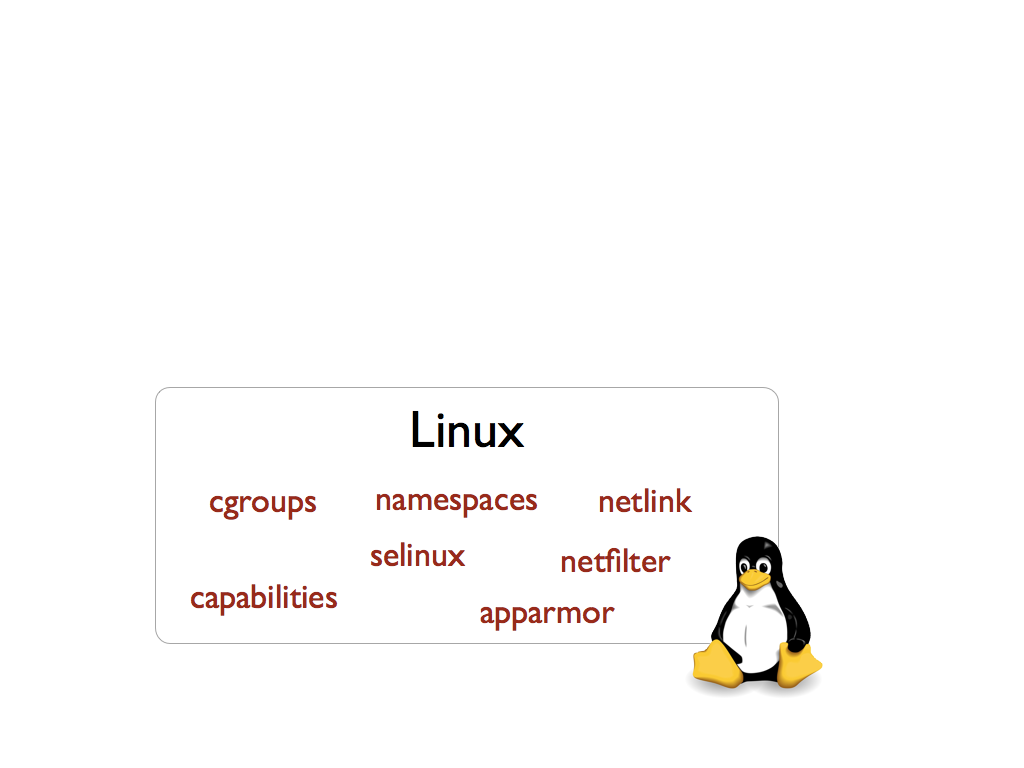
\includegraphics[width=1\linewidth]
            {img/docker_diagram_kernel.png}
    }
    \only<2>{
        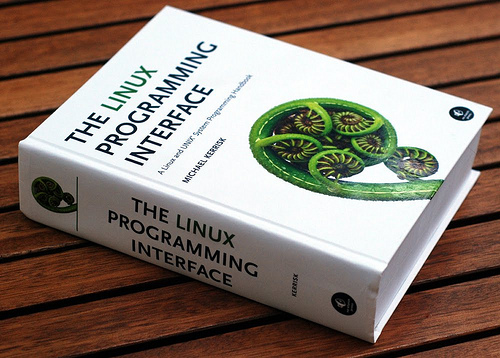
\includegraphics[width=0.8\linewidth]
            {img/the-linux-programming-interface.jpg}
    }
    \only<3>{
        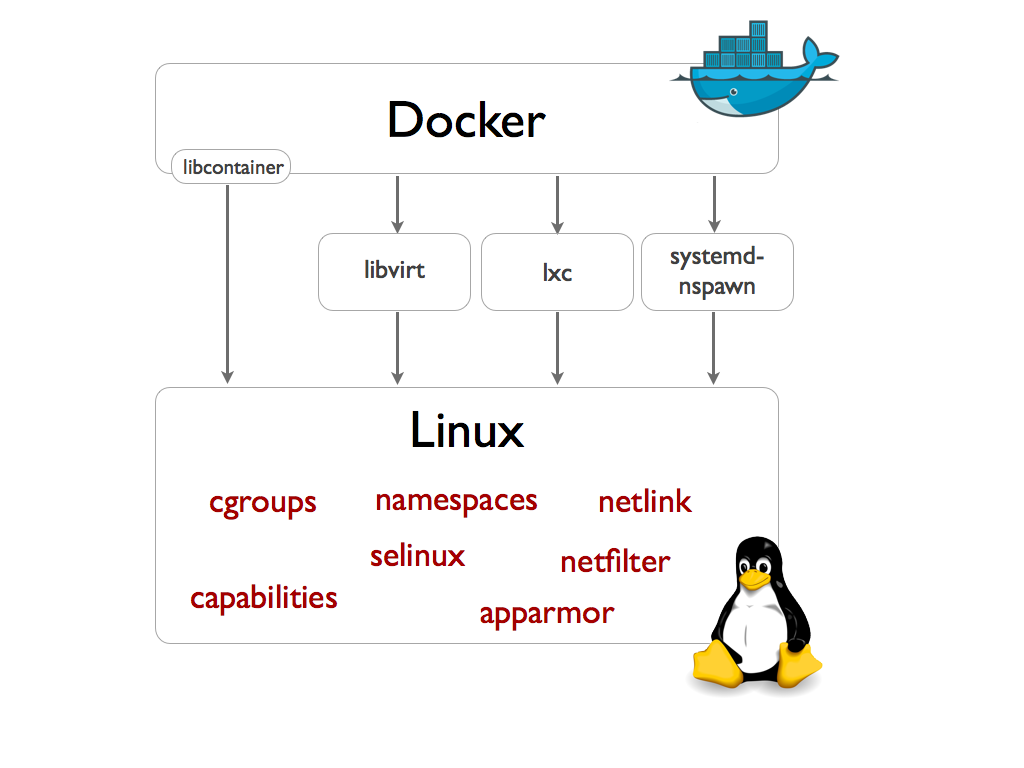
\includegraphics[width=1\linewidth]
            {img/docker-execdriver-diagram.png}
    }
    \note<1>{
        Most of the tools that are used to implement containers have been in
        the kernel for years.
    }
    \note<2>{
        But those are low-level tools that require some level of systems
        programming.
    }
    \note<3>{
        The change that led to the recent popularization of containers was the
        development of systems that make use of these tools while providing a
        user (or developer) interface that is much simpler, inspired by web
        application development.  Dotcloud, before becoming Docker, was a PaaS
        company.
    }
\end{frame}

\subsection{pros-cons}

\subsubsection{pros}

\begin{frame}
    \autotitle
    \begin{itemize}
        \item new and highly expanding technologies
        \item shared kernel
            \begin{itemize}
                \item hardware is not virtualized
                \begin{itemize}
                    \item smaller overhead
                    \item smaller resource utilization
                \end{itemize}
                \item faster initialization (\textit{ms})
                \item single update
                    (\textit{kpatch}/\textit{ksplice}/\textit{live patching}?)
            \end{itemize}
    \end{itemize}
\end{frame}

\subsubsection{cons}

\begin{frame}
    \autotitle
    \begin{itemize}
        \item new and highly expanding technologies
        \item shared kernel
        \begin{itemize}
            \item hardware is not virtualized
            \item only one type
            \begin{itemize}
                \item version
                \item architecture
                \item operating system
            \end{itemize}
            \item kernel exploits
        \end{itemize}
    \end{itemize}
\end{frame}

\begin{frame}
    \autotitle
    \begin{quote}
        There’s an additional advantage to containerizing your application. It
        forces you to think hard about configuration, limiting the amount of
        mutable state inside your environment and your ability to scale
        horizontally.
        \\~\\
        An exercise in switching to container-based deploys is actually an
        exercise in good engineering practices and any extra work required by
        Docker pays off by making your codebase better factored and less
        brittle.
    \end{quote}
    Jan Urbański - New Relic
\end{frame}

\section{implementation}

\begin{frame}
    \autotitle
    \begin{itemize}
        \item cgroups
        \item namespaces
    \end{itemize}
\end{frame}

\subsection{cgroups}

\begin{frame}
    \autotitle
    \begin{itemize}
        \item linux 2.6.24 (2007)
        \item resource limiting/reservation
        \item accounting/auditing
    \end{itemize}
\end{frame}

\begin{frame}[fragile]
    \autotitle
    \verb|awk 'NR>1{print$1}' /proc/cgroups|
    \begin{multicols}{3}
        \begin{itemize}
            \item cpuset
            \item cpu
            \item cpuacct
            \item blkio
            \item memory
            \item devices
            \item freezer
            \item net\_cls
            \item pids
        \end{itemize}
    \end{multicols}
\end{frame}

\begin{frame}[fragile]
    \autotitle
    \begin{verbatim}
$ awk '/cgroup/{sub(".*,","",$4);print$2,$3,$4}' /proc/mounts
/sys/fs/cgroup tmpfs mode=755
/sys/fs/cgroup/systemd cgroup name=systemd
/sys/fs/cgroup/blkio cgroup blkio
/sys/fs/cgroup/cpu,cpuacct cgroup cpuacct
/sys/fs/cgroup/net_cls cgroup net_cls
/sys/fs/cgroup/pids cgroup pids
/sys/fs/cgroup/cpuset cgroup cpuset
/sys/fs/cgroup/devices cgroup devices
/sys/fs/cgroup/freezer cgroup freezer
/sys/fs/cgroup/memory cgroup memory
    \end{verbatim}
\end{frame}

\subsubsection{cpuset}

\begin{frame}[fragile]
    \autotitle
    \begin{itemize}
        \item \verb|cat /sys/fs/cgroup/cpuset/cpuset.mems|
        \item \verb|echo 0-1 > /sys/fs/cgroup/cpuset/cpuset.mems|
        \item \verb|cat /sys/fs/cgroup/cpuset/cpuset.cpus|
        \item \verb|echo 3-5 > /sys/fs/cgroup/cpuset/cpuset.cpus|
    \end{itemize}
\end{frame}

\subsubsection{cpu}

\begin{frame}[fragile]
    \autotitle
    \begin{itemize}
        \item \verb|cat /sys/fs/cgroup/cpu/cpu.shares|
        \item \verb|echo 1024 > /sys/fs/cgroup/cpu/cpu.shares|
    \end{itemize}
\end{frame}

\subsubsection{cpuacct}

\begin{frame}[fragile]
    \autotitle
    \begin{itemize}
        \item \verb|cat /sys/fs/cgroup/cpuacct/cpuacct.stat|
        \item \verb|cat /sys/fs/cgroup/cpuacct/cpuacct.usage|
        \item \verb|cat /sys/fs/cgroup/cpuacct/cpuacct.usage_percpu|
    \end{itemize}
\end{frame}

\subsubsection{blkio}

\begin{frame}[fragile]
    \autotitle
    \verb!ls /sys/fs/cgroup/blkio/blkio.* | grep -v '_recursive'!
    \begin{multicols}{2}
        \begin{itemize}
            \item blkio.io\_merged
            \item blkio.io\_queued
            \item blkio.io\_service\_bytes
            \item blkio.io\_serviced
            \item blkio.io\_service\_time
            \item blkio.io\_wait\_time
            \item blkio.leaf\_weight
            \item blkio.leaf\_weight\_device
            \item blkio.reset\_stats
            \item blkio.sectors
            \item blkio.throttle.io\_service\_bytes
            \item blkio.throttle.io\_serviced
            \item blkio.throttle.read\_bps\_device
            \item blkio.throttle.read\_iops\_device
            \item blkio.throttle.write\_bps\_device
            \item blkio.throttle.write\_iops\_device
            \item blkio.time
            \item blkio.weight
            \item blkio.weight\_device
        \end{itemize}
    \end{multicols}
\end{frame}

\subsubsection{memory}

\begin{frame}[fragile]
    \autotitle
    \begin{itemize}
        \item \verb|cat /sys/fs/cgroup/memory/memory.usage_in_bytes|
        \item \verb|cat /sys/fs/cgroup/memory/memory.limit_in_bytes|
        \item \verb|echo $x > /sys/fs/cgroup/memory/memory.limit_in_bytes|
    \end{itemize}
\end{frame}

\begin{frame}[fragile]
    \autotitle
    \verb|awk '!/^total_/{print$1}' /sys/fs/cgroup/memory/memory.stat|
    \begin{multicols}{2}
        \begin{itemize}
            \item cache
            \item rss
            \item rss\_huge
            \item mapped\_file
            \item dirty
            \item writeback
            \item swap
            \item pgpgin
            \item pgpgout
            \item pgfault
            \item pgmajfault
            \item inactive\_anon
            \item active\_anon
            \item inactive\_file
            \item active\_file
            \item unevictable
            \item hierarchical\_memory\_limit
            \item hierarchical\_memsw\_limit
        \end{itemize}
    \end{multicols}
\end{frame}

\subsubsection{devices}

\begin{frame}[fragile]
    \autotitle
    \begin{itemize}
        \item \verb|cat /sys/fs/cgroup/devices/devices.list|
        \item \verb|echo 'a *:* rwm' > /sys/fs/cgroup/devices/devices.allow|
        \item \verb|echo a > /sys/fs/cgroup/devices/devices.deny|
    \end{itemize}
\end{frame}

\subsubsection{freezer}

\begin{frame}[fragile]
    \autotitle
    \begin{itemize}
        \item \verb|cat /sys/fs/cgroup/$child/freezer.state|
        \item \verb|echo FROZEN> /sys/fs/cgroup/$child/freezer.state|
        \item \verb|echo THAWED > /sys/fs/cgroup/$child/freezer.state|
    \end{itemize}
\end{frame}

\subsubsection{net\_cls}

\begin{frame}[fragile]
    \autotitle
    \begin{itemize}
        \item \verb|cat /sys/fs/cgroup/net_cls/net_cls.classid|
        \item \verb|maj=0001; min=0001; cls=0x$maj$min|
        \item \verb|echo $cls > /sys/fs/cgroup/net_cls/net_cls.classid|
    \end{itemize}
\end{frame}

\subsubsection{pid}

\begin{frame}[fragile]
    \autotitle
    \begin{itemize}
        \item \verb|cat /sys/fs/cgroup/pids/pids.current|
        \item \verb|echo 2 > /sys/fs/cgroup/pids/pids.max|
    \end{itemize}
\end{frame}

\subsection{namespaces}

\begin{frame}
    \autotitle
    \begin{itemize}
        \only<1>{
            \item \texttt{unshare(2)}
            \item \texttt{clone(2)}
            \item \texttt{setns(2)}
        }
        \only<2>{
            \item mnt (\texttt{CLONE\_NEWNS})
            \item uts (\texttt{CLONE\_NEWUTS})
            \item ipc (\texttt{CLONE\_NEWIPC})
            \item pid (\texttt{CLONE\_NEWPID})
            \item net (\texttt{CLONE\_NEWNET})
            \item uid (\texttt{CLONE\_NEWUSER})
        }
    \end{itemize}
    \note<1>{
        Namespaces are an isolation facility provided by the kernel.  They are
        at the core of containers and are responsible for the isolation that
        allows processes to execute on the same machine without interfering
        with each other.
        \\~\\
        Namespaces can be manipulated using three system calls:
        \begin{itemize}
            \item
                \texttt{unshare(2)} creates a namespace and associates the
                process to it.
            \item
                \texttt{clone(2)} is similar to a \texttt{fork(2)} followed by
                an \texttt{unshare(2)}.
            \item
                \texttt{setns(2)} associates a process with an existing
                namespace.
        \end{itemize}
    }
    \note<2>{
        Each of this syscalls takes a \texttt{flag} argument which includes
        these values for selecting which namespace(s) should created/joined.
    }
\end{frame}

\subsubsection{mount}

\begin{frame}
    \autotitle
    \begin{itemize}
        \item \texttt{CLONE\_NEWNS}
        \item linux 2.4.19 (2002)
        \item \texttt{mount(2)/umount(2)}
        \item different processes have different visions of the file system
        \item ``\texttt{chroot(2)} on steroids''
        \item sharing of mount points
    \end{itemize}
\end{frame}

\subsubsection{uts}

\begin{frame}
    \autotitle
    \begin{itemize}
        \item \texttt{CLONE\_NEWUTS}
        \item linux 2.6.19 (2006)
        \item \texttt{uname(2)}
        \item \texttt{sethotname(2)}
        \item \texttt{setdomainname(2)}
        \item Unix Timesharing System
    \end{itemize}
\end{frame}

\subsubsection{ipc}

\begin{frame}
    \autotitle
    \begin{itemize}
        \item \texttt{CLONE\_NEWIPC}
        \item linux 2.6.19 (2006) / linux 2.6.30 (2009)
        \item \texttt{svipc(7)}/\texttt{mq\_overview(7)}
        \item isolation for the 32-bit resource ids
        \item
            sysV IPC has been mostly superseded, but some programs (e.g.
            postgresql) still use it
    \end{itemize}
\end{frame}

\subsubsection{pid}

\begin{frame}
    \autotitle
    \begin{itemize}
        \item \texttt{CLONE\_NEWPID}
        \item linux 2.6.24 (2008)
        \item each pid inside a namespace is mapped to a pid outside
        \item the same pid may appear on different namespaces
        \item processes don't see processes of other namespaces
        \item
            offers protection from pid-based syscalls like \texttt{kill(2)},
            \texttt{ptrace(2)}, etc
        \item
            \texttt{procfs} only shows information related to processes on the
            namespace
        \item migration between hosts
        \item each namespace has its own pid 1
        \item
            can be nested: a parent namespace can see and affect processes on
            child namespaces; processes on a child namespace don't see and
            can't do anything to processes on the parent
    \end{itemize}
\end{frame}

\subsubsection{net}

\begin{frame}
    \autotitle
    \begin{itemize}
        \item \texttt{CLONE\_NEWNET}
        \item linux 2.6.24 (2008)
        \item each namespace has its own
            \begin{itemize}
                \item network devices (including \texttt{lo})
                \item ip addresses
                \item routing tables
                \item \texttt{/proc/net}
                \item ports
                \item etc.
            \end{itemize}
        \item
            communication with the host or with other namespaces can be
            implemented using \texttt{veth} pairs and/or bridge interfaces
        \item
            \texttt{INADDR\_ANY} (a.k.a. \texttt{0.0.0.0}) means "any address
            on the current namespace"
    \end{itemize}
\end{frame}

\subsubsection{user}

\begin{frame}
    \autotitle
    \begin{itemize}
        \item \texttt{CLONE\_NEWUSER}
        \item linux 2.6.23 (2007)
        \item finalized on kernel 3.8 (2013) $->$ $\sim$ five years
        \item uid and gid isolation and mapping
        \item \texttt{uid 0}
        \item recursive
        \begin{itemize}
            \item an unprivileged process can create a namespace
            \item \texttt{uid 0} inside the namespace
            \item<2> ö
        \end{itemize}
    \end{itemize}
\end{frame}

\subsubsection{demo}

\begin{frame}[fragile]
    \autotitle
    \begin{semiverbatim}
        \only<1>{
# create containers
./ns_test
# create pairs of veths
ip link add h1 type veth peer name c1
ip link add h2 type veth peer name c2
# move one to each container's namespace
ip link set dev c1 netns /proc/$pid1/ns/net
ip link set dev c2 netns /proc/$pid2/ns/net
# rename each container's veth to eth0
nsenter --net --target $pid1 ip link set dev c1 name eth0
nsenter --net --target $pid2 ip link set dev c2 name eth0
        }
        \only<2>{
# assign addresses to each container's interfaces
nsenter -n -t $pid1 ip addr add 10.0.0.2/8 dev eth0
nsenter -n -t $pid2 ip addr add 10.0.0.3/8 dev eth0
nsenter -n -t $pid1 ip set eth0 up
nsenter -n -t $pid2 ip set eth0 up
ip link set h1 up
ip link set h2 up
# create a bridge and add the containers' interfaces
brctl addbr br0
brctl addif br0 h1 h2
        }
    \end{semiverbatim}
    \note<1>{
        This demo shows how multiple network namespaces can all be connected.
        Outside the namespaces, for each container:
        \begin{itemize}
            \item a pair of \texttt{veth}'s is created
            \item one of the endpoints is moved to the network namespace
            \item the interface name inside the namespace is changed to "eth0"
            \item an address is assigned to it
        \end{itemize}
        Finally, a bridge interface is created and the other endpoints of all
        the pairs are added to it.  This bridge routes packets coming from/to
        the veth pairs as if they were connected by a layer 2 hub.
    }
\end{frame}

\begin{frame}[fragile]
    \autotitle
    \begin{figure}
        \centering
        \begin{varwidth}{\linewidth}
            \begin{verbatim}
 -- container0 --   -- container1 --
|      eth0      | |      eth0      |
 --------|-------   --------|-------
         |                  |
 --------|------ br0 -------|-------
|        h1                 h2      |
 -----------------------------------
            \end{verbatim}
        \end{varwidth}
    \end{figure}
\end{frame}

\section{security}

\subsection{root}

\begin{frame}
    \autotitle
    \only<1>{
        \begin{itemize}
            \item don't use
        \end{itemize}
    }
    \only<2>{
        \begin{quote}
            For repos we recognize on or after 2015-01-01, linux builds are
            sent to our container-based infrastructure.
        \end{quote}
        Travis CI
    }
    \only<3>{
        \begin{quote}
            This job is running on container-based infrastructure, which
            does not allow use of 'sudo', setuid and setguid executables.
            If you require sudo, add 'sudo: required' to your .travis.yml
        \end{quote}
        Travis CI
    }
\end{frame}

\subsection{applications}

\begin{frame}
    \autotitle
    \begin{itemize}
        \item
            Most containers execute a specific task, instead of a complete
            system, and most applications (\textit{apache}, \textit{nginx},
            \textit{postgresql}, \textit{redis}, ...) don't need \textit{root}
            privileges.
        \item
            The risks are the same as before: assume the application can do
            anything to escape isolation.
    \end{itemize}
\end{frame}

\begin{frame}
    \autotitle
    \only<1>{
        syscalls
        \begin{itemize}
            \item e.g. \texttt{vmsplice(2)}
            \item limits the \textit{syscalls} available
            \item seccomp/seccomp-bpf
            \item \texttt{capabilities(7)}
            \item \texttt{selinux(8)}/\texttt{apparmor(7)}
            \item grsec
            \item constant updates
        \end{itemize}
        = reduce kernel exposure
    }
    \only<2>{
        \begin{quote}
            ``[...] there's maybe marginal increases in practical security for
            certain kinds of deployment, and perhaps marginal decreases for
            others.  We end up coming back to the attack surface, and it seems
            inevitable that that's always going to be larger in container
            environments. The question is, does it matter? If the larger attack
            surface still only results in one more vulnerability per thousand
            years, you probably don't care. The aim isn't to get containers to
            the same level of security as hypervisors, it's to get them close
            enough that the difference doesn't matter.''
        \end{quote}
        Matthew Garrett
    }
    \note<1>{
        The big difference in the surface of attack between virtual machines
        and containers is the kernel.  On a virtual machine, an attacker that
        is able to exploit the (guest) kernel still has to break out to the
        hypervisor.  Since containers share the same kernel, an exploit gives
        direct access to the system.
        \\~\\
        Since the interface to the kernel is the system calls, a big part in
        securing containers involves hardening them.  Although kernel exploits
        are rare, they exist: the \texttt{vmsplice} one is a recent example.
        Limiting the syscalls available can be done using the \texttt{seccomp}
        family of syscalls.  Capabilities, selinx and apparmor reduce the
        impact of an exploit by clearly delimiting the actions a process can
        take.  The grsec kernel is a series of out-of-tree patches that
        prioritize security.
    }
\end{frame}

\section{references}

\begin{frame}
    \autotitle
    \begin{itemize}
        \item
            \href
                {https://blog.newrelic.com/2015/06/18/zero-to-docker/}
                {Zero to docker}
        \item
            \href
                {https://www.kernel.org/doc/Documentation/cgroups-v1/}
                {cgroups docs}
        \item
            \href
                {https://www.kernel.org/doc/Documentation/cgroups-v2.txt}
                {cgroups-v2 docs}
        \item
            \href
                {https://lwn.net/Articles/531114/}
                {Namespaces in operation}
        \item
            \href
                {http://mjg59.dreamwidth.org/33170.html}
                {Linux Container Security}
        \item
            \href
                {http://www.slideshare.net/jpetazzo/docker-linux-containers-lxc-and-security}
                {Docker, Linux Containers (LXC), and security}
        \item
            \href
                {https://lwn.net/Articles/268783/}
                {vmsplice(): the making of a local root exploit}
        \item
            \href
                {https://www.youtube.com/watch?v=0T2XFSALOaU}
                {Docker in Production: Tales From the Engine Room [video]}
    \end{itemize}
\end{frame}

\begin{frame}
    \autotitle
    \begin{itemize}
        \item
            \href
                {http://www.servicioswebgratis.com/wp-content/uploads/2012/08/the-linux-programming-interface.jpg}
                {The Linux Programming Interface}
        \item
            \href
                {http://blog.docker.com/2014/03/docker-0-9-introducing-execution-drivers-and-libcontainer/}
                {Docker drivers}
    \end{itemize}
\end{frame}

\end{document}
